\documentclass[11pt,a4paper]{article}

\usepackage[utf8]{inputenc}
\usepackage{amsmath, amssymb, amsfonts}
\usepackage{graphicx}
\usepackage{hyperref}
\usepackage{geometry}
\usepackage{float}
\usepackage{booktabs}
\usepackage{caption}
\usepackage{subcaption}

\geometry{margin=1in}

\title{\textbf{Overestimation Bias in Value-Based RL: From Q-Learning to Double DQN}}
\author{FRA503 Deep Reinforcement Learning Final Project}
\date{\today}

\begin{document}

\maketitle

\section{Project Overview}
Value-based Reinforcement Learning (RL) relies heavily on estimating the expected return of actions to derive optimal policies. The cornerstone algorithm, Q-Learning, utilizes the $\max$ operator to estimate the value of the next state. While mathematically elegant, this introduces a systematic overestimation bias because the maximum of noisy estimates is consistently greater than the true maximum expected value. Over time, this positive bias can compound, leading to suboptimal policies. This project aims to empirically observe, measure, and analyze this overestimation bias, transitioning from simple Tabular RL to complex Deep RL using neural network function approximation.

\section{Scope Revision and Objectives}
The original project proposal was titled ``Overestimation Bias in Value-Based RL: From Q-Learning to Double DQN with Prioritized Experience Replay''. The initial scope included the implementation of Prioritized Experience Replay (PER). However, during the implementation of the Deep RL experiments, a more fundamental stability problem emerged: the \textit{Deadly Triad}. Function approximation combined with bootstrapping and off-policy learning caused the Q-values to diverge massively. 

Consequently, the final project scope was revised. The implementation of PER was moved to Future Work. The revised scope focuses on hyperparameter tuning to mitigate the Deadly Triad instability, enabling a stable environment to accurately measure the underlying overestimation bias in Deep Q-Networks (DQN) and Double DQN. The primary objective is to evaluate whether the Double estimator approach reduces overestimation across both Tabular and Deep RL settings.

\section{Research Questions}
This study is guided by the following core research questions:
\begin{enumerate}
    \item \textbf{RQ1:} Does Q-Learning exhibit positive overestimation bias in a tabular setting?
    \item \textbf{RQ2:} Can Double Q-Learning reduce the positive bias caused by the max operator?
    \item \textbf{RQ3:} After stabilizing Deep RL training, does Double DQN reduce MaxQ Bias compared to DQN?
\end{enumerate}

\section{Theoretical Background}
\subsection{Value-Based Reinforcement Learning}
Value-based methods aim to learn the optimal action-value function $Q^*(s,a)$, which represents the maximum expected cumulative reward achievable from state $s$ by taking action $a$.

\subsection{Overestimation Bias and the Max Operator}
The standard Q-Learning update rule is:
\begin{equation}
    Q(s,a) \leftarrow Q(s,a) + \alpha \left[ r + \gamma \max_{a'} Q(s',a') - Q(s,a) \right]
\end{equation}
The root cause of overestimation lies in the target $r + \gamma \max_{a'} Q(s',a')$. Let $X$ be the noisy estimate of the true value. Due to Jensen's inequality and the convexity of the max function, we have:
\begin{equation}
    \mathbb{E}[\max(X)] \ge \max(\mathbb{E}[X])
\end{equation}
Using the same noisy Q-table to both \textit{select} the best action and \textit{evaluate} its value introduces a positive bias, as the estimator is more likely to select actions whose values are currently overestimated by noise.

\subsection{Double Estimator and Double Q-Learning}
Double Q-Learning decouples selection and evaluation using two separate tables ($Q_A$ and $Q_B$). If $Q_A$ is used to select the action $a^* = \arg\max_a Q_A(s', a)$, then $Q_B$ is used to evaluate it: $Q_B(s', a^*)$. This breaks the positive feedback loop and mitigates the accumulation of overestimation bias.

\subsection{Deep Q-Networks and Double DQN}
DQN extends Q-Learning by employing a feedforward neural network, an experience replay buffer, and a slowly updating target network. Double DQN (DDQN) adapts the double estimator concept by using the online network to select the action and the target network to evaluate it.

\subsection{Deadly Triad in Deep RL}
The \textit{Deadly Triad} describes the instability and potential for divergence when three elements are combined: Function Approximation (e.g., Neural Networks), Bootstrapping (updating estimates based on other estimates), and Off-policy learning (learning from an experience replay buffer). 

\section{Methodology}
\subsection{Algorithms}
Four algorithms were implemented to trace the evolution of the bias: Tabular Q-Learning, Tabular Double Q-Learning, Deep Q-Network (DQN), and Double DQN (DDQN).

\subsection{MaxQ Bias Measurement using Monte Carlo Return}
To empirically measure bias, we define our primary metric:
\begin{equation}
    \text{MaxQ Bias}(s_t) = \max_a Q(s_t, a) - G_t^{MC}
\end{equation}
where $G_t^{MC}$ is the actual Monte Carlo return achieved by following a greedy policy from state $s_t$. Because Monte Carlo return is calculated without bootstrapping, it serves as an empirical reference return for comparing Q-value estimates. Positive values indicate overestimation, while negative values indicate underestimation. It should be noted that in Deep RL settings, the Monte Carlo return can be noisy and may be affected by function approximation and replay buffer mismatch.

\subsection{Hyperparameter Tuning Strategy}
To make the Deep RL comparison meaningful, hyperparameter tuning was applied after initial DQN and Double DQN training showed severe Q-value divergence. The purpose of this tuning process was not to optimize final reward directly, but to stabilize learning enough for MaxQ Bias to be measured reliably. The following stabilizing changes were applied:
\begin{itemize}
    \item Target update interval: 1000 $\rightarrow$ 100
    \item Discount factor $\gamma$: 0.99 $\rightarrow$ 0.95
    \item Gradient clipping: 10.0 $\rightarrow$ 1.0
    \item Minimum replay buffer size: 1000 $\rightarrow$ 5000
\end{itemize}

\section{Experiment Design and Setup}

\subsection{Environment and MDP Formulation}
All experiments were conducted on the \texttt{Stabilize-Isaac-Cartpole-v0} environment in IsaacLab. The observation state consists of continuous variables: cart position, pole angle, cart velocity, and pole angular velocity. For tabular algorithms, this space was discretized into bins $[8, 16, 8, 8]$. The action space is discrete, offering five force levels: $[-1.0, -0.5, 0.0, 0.5, 1.0]$. 

\subsection{Evaluation Metrics}
\begin{itemize}
    \item \textbf{Primary Metric:} \textit{MaxQ Bias}.
    \item \textbf{Secondary Metrics:} Average Reward (policy performance), Episode Duration (stability), Action Distribution (behavior), and Pole Angle Trajectory (smoothness).
\end{itemize}

Experiments were run across 5 random seeds to improve reliability across random initializations. Evaluation was performed via Greedy Evaluation, where exploration ($\epsilon$) was disabled to accurately collect empirical Monte Carlo returns without exploratory noise.

\subsection{Experiment 1: Tabular RL}
This experiment compares Q-Learning and Double Q-Learning in a discretized tabular setting. The objective is to isolate the max-operator effect without the additional complexity of neural network function approximation. Since tabular Q-values are directly observable, this experiment serves as a controlled baseline for evaluating whether Q-Learning produces positive MaxQ Bias and whether Double Q-Learning reduces this bias.

\subsection{Experiment 2: Deep RL}
This experiment extends the analysis from tabular value estimation to neural network function approximation by comparing DQN and Double DQN. The objective is to examine whether the double estimator idea still reduces MaxQ Bias when Q-values are approximated by neural networks. 

During the initial implementation, however, the combination of function approximation, bootstrapping, and off-policy replay caused severe Q-value divergence. Therefore, the Deep RL results are reported in two parts in the Results section: first, the unstable result before hyperparameter tuning is shown as a diagnostic observation; second, the stabilized result after hyperparameter tuning is used as the main DQN vs Double DQN comparison.

\section{Results}

\subsection{Experiment 1: Tabular RL Results}

\begin{figure}[H]
    \centering
    \begin{subfigure}{0.48\textwidth}
        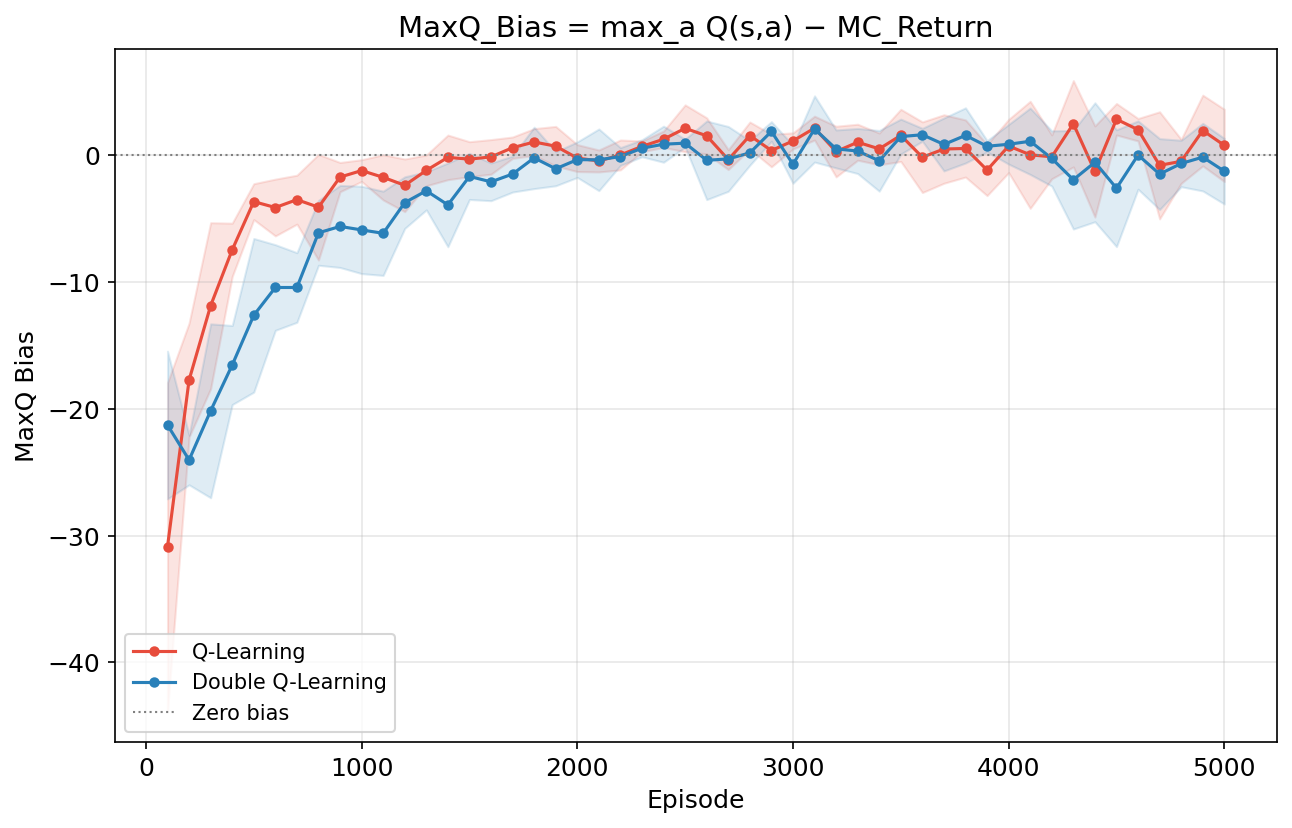
\includegraphics[width=\linewidth]{report_figures/phase1_maxq_bias_curve.png}
    \end{subfigure}
    \hfill
    \begin{subfigure}{0.48\textwidth}
        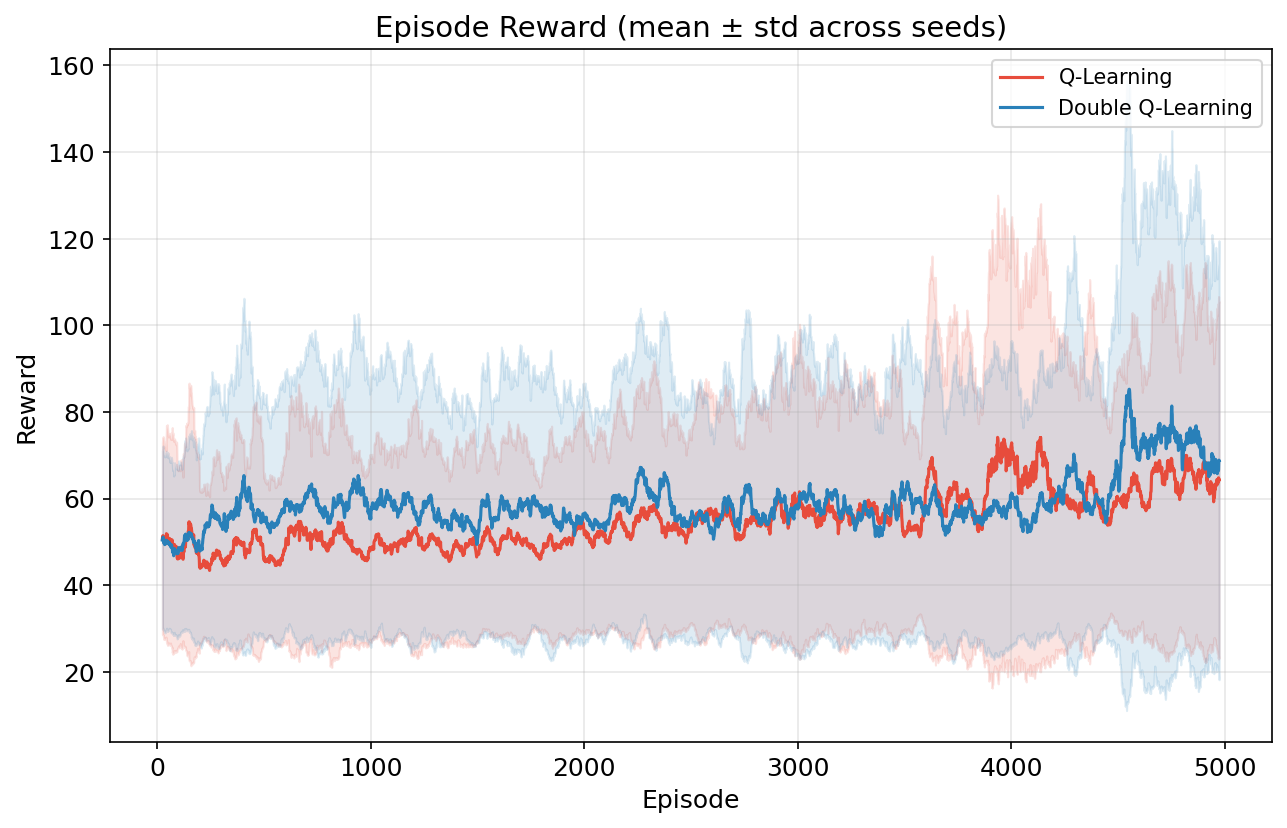
\includegraphics[width=\linewidth]{report_figures/phase1_reward_curve.png}
    \end{subfigure}
    \caption{MaxQ Bias and Average Reward in Tabular RL}
    \label{fig:exp1_bias}
\end{figure}

As training progresses in the tabular environment, Q-Learning gradually develops a positive MaxQ Bias (+0.796), suggesting that the max operator systematically inflates value estimates. In contrast, Double Q-Learning remains largely in the negative domain (-1.241), indicating that decoupling action selection and evaluation reduces positive overestimation. The average reward curves show that Double Q-Learning achieves a slightly higher final average reward (67.59) compared to Q-Learning (63.08), suggesting that reducing overestimation bias can also improve policy quality in this tabular setting. However, Q-Learning exhibits wider variance across seeds, particularly in the later episodes, indicating that overestimation may make the policy more sensitive to random initialization.

\vspace{1em}

\begin{figure}[H]
    \centering
    \begin{subfigure}{0.48\textwidth}
        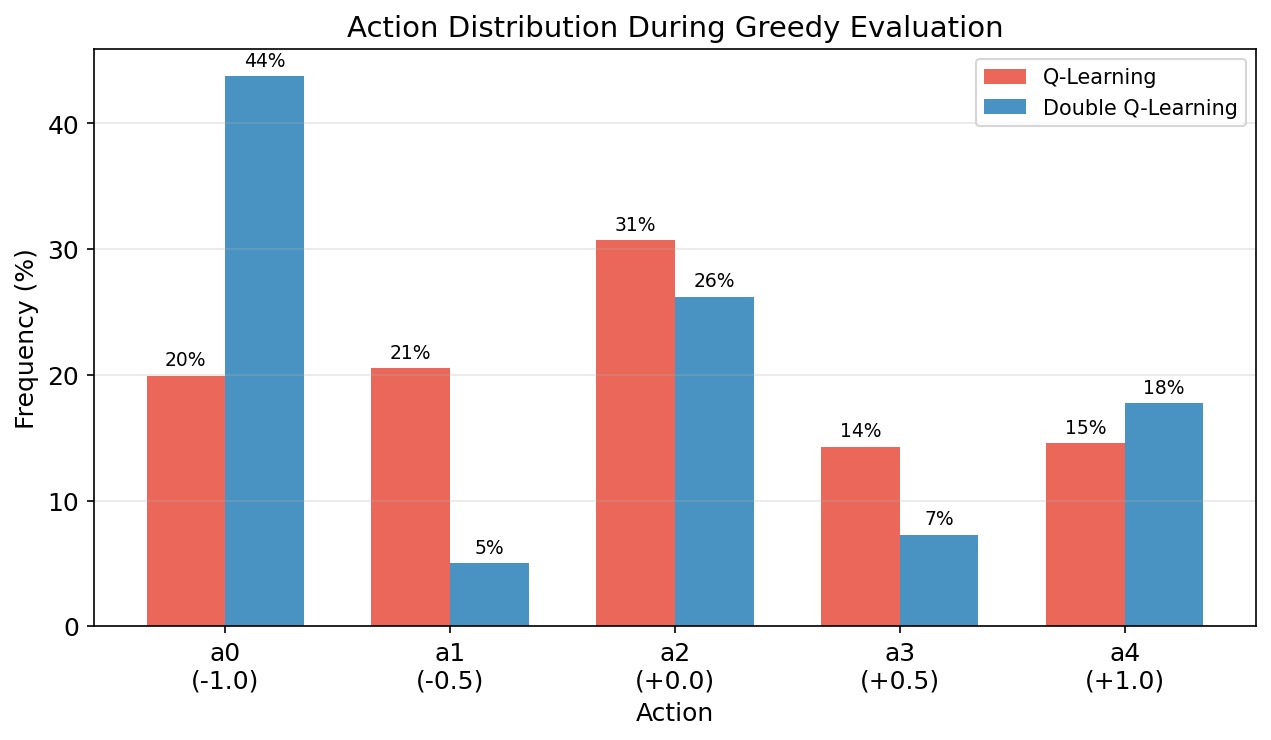
\includegraphics[width=\linewidth]{report_figures/phase1_action_distribution.png}
    \end{subfigure}
    \hfill
    \begin{subfigure}{0.48\textwidth}
        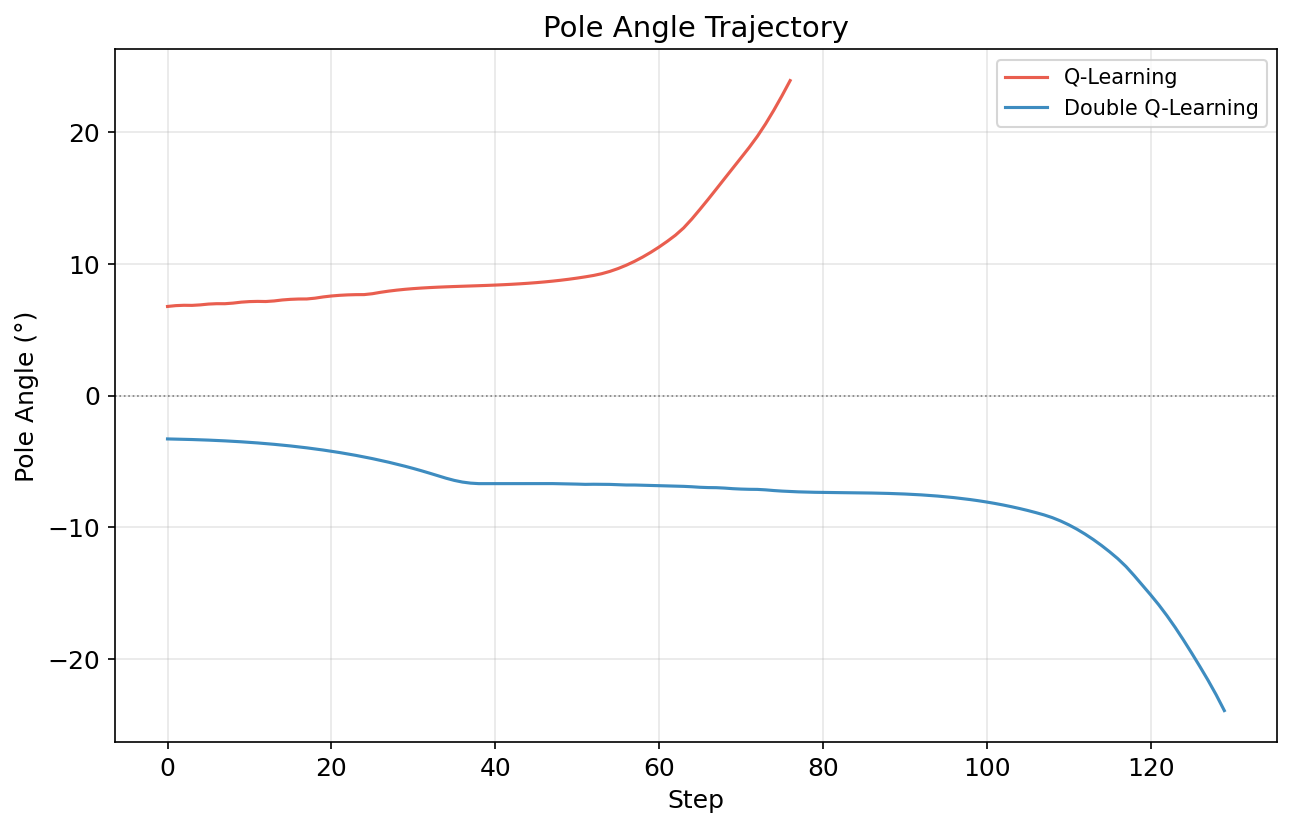
\includegraphics[width=\linewidth]{report_figures/phase1_pole_angle_trajectory.png}
    \end{subfigure}
    \caption{Action Distribution and Pole Angle Behavior in Tabular RL}
    \label{fig:exp1_behavior}
\end{figure}

The action distribution and pole angle trajectory reveal distinct behavioral differences between the two tabular methods. Q-Learning does not appear to be more aggressive; rather, its action choices are more spread across all five force levels and include a noticeable tendency toward the neutral action ($a_2 = 0.0$ at 31\%), suggesting delayed correction. This causes the pole angle to drift before effective intervention is applied, leading to earlier failure in the greedy evaluation. In contrast, Double Q-Learning concentrates heavily on the strongest corrective action ($a_0 = -1.0$ at 44\%), which better compensates for the initial pole angle and allows the pole to remain balanced for a longer duration. These diagnostic metrics suggest that reducing overestimation bias changes not only the value estimates but also the learned control behavior.

\subsection{Deep RL before Hyperparameter Tuning: Stability Diagnostic}

\begin{figure}[H]
    \centering
    \begin{subfigure}{0.48\textwidth}
        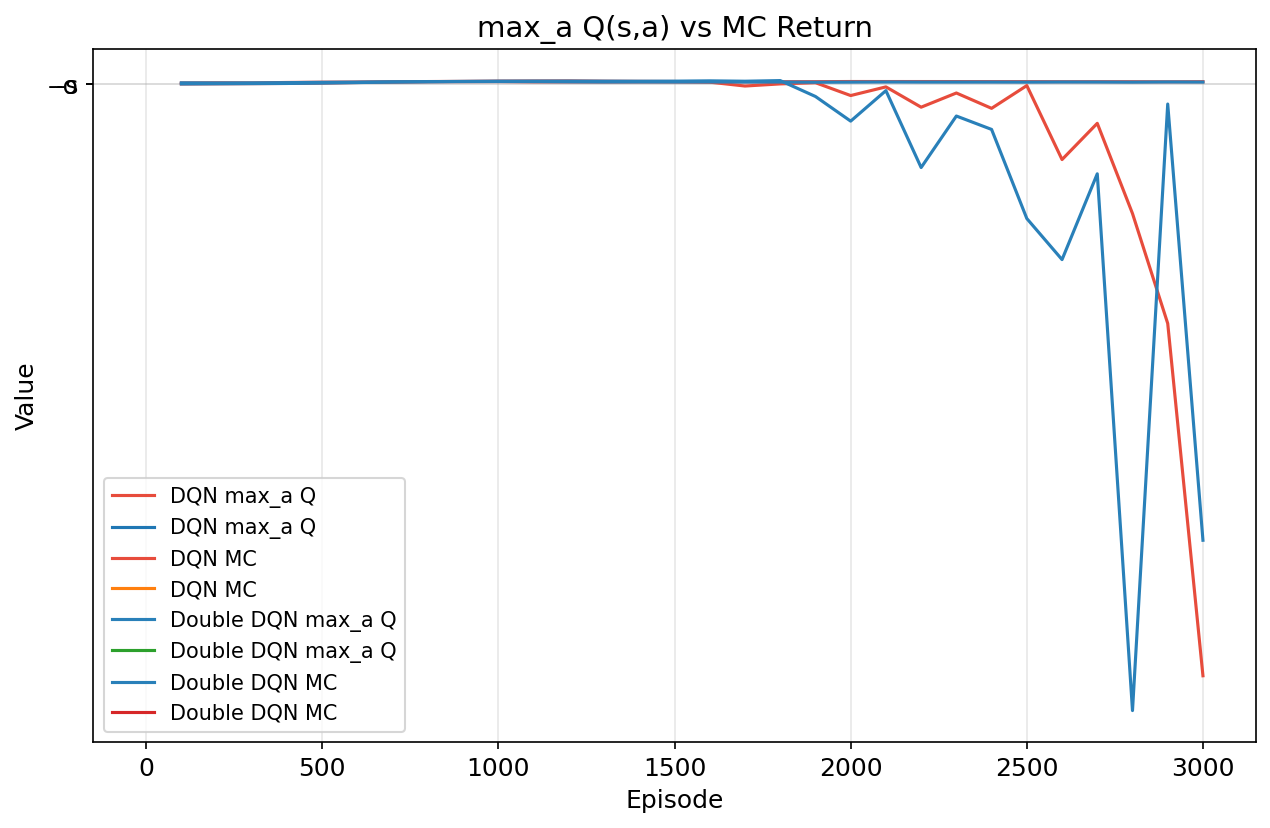
\includegraphics[width=\linewidth]{report_figures/phase2_before_q_divergence.png}
    \end{subfigure}
    \hfill
    \begin{subfigure}{0.48\textwidth}
        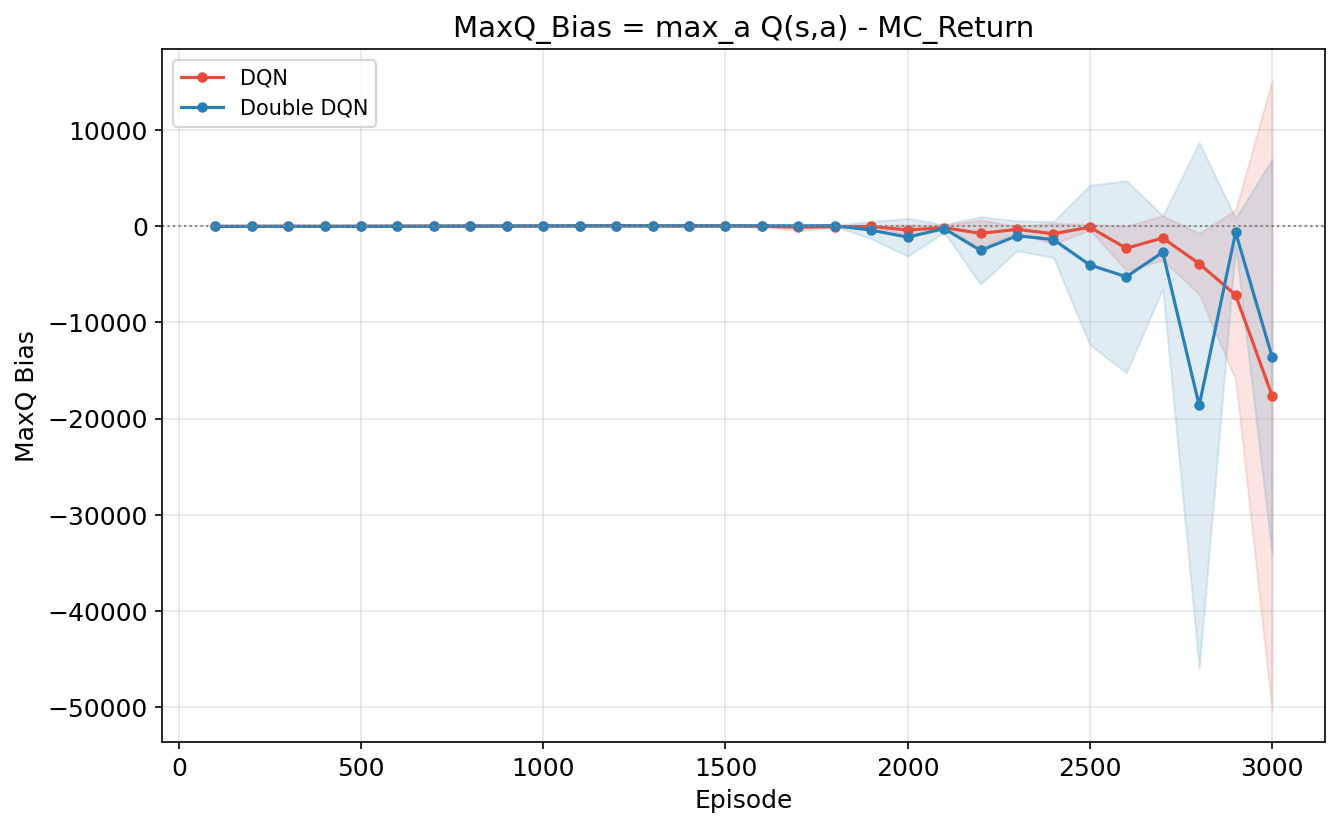
\includegraphics[width=\linewidth]{report_figures/phase2_before_maxq_bias_curve.png}
    \end{subfigure}
    \caption{Q-Value Divergence and MaxQ Bias before Tuning}
    \label{fig:exp2_divergence}
\end{figure}

Before applying stabilizing hyperparameter adjustments, both DQN and Double DQN failed to show meaningful overestimation behavior due to fundamental network instability. The Q-values collapsed into extreme negative ranges, with DQN reaching approximately -17,539 and Double DQN reaching approximately -13,582, causing severe underestimation in both cases. The results in this diagnostic observation are heavily influenced by Deadly Triad instability rather than the intended max-operator effect. Notably, Double DQN diverged less severely than standard DQN, suggesting that the double estimator may partially slow the error accumulation even under unstable conditions.

The pre-tuning result shows that the Deep RL comparison could not be interpreted as a clean overestimation-bias analysis because the Q-values were dominated by instability. Therefore, hyperparameter tuning was applied to reduce divergence and create a more stable condition for comparing DQN and Double DQN.

\subsection{Deep RL after Hyperparameter Tuning: DQN vs Double DQN}

\begin{figure}[H]
    \centering
    \begin{subfigure}{0.48\textwidth}
        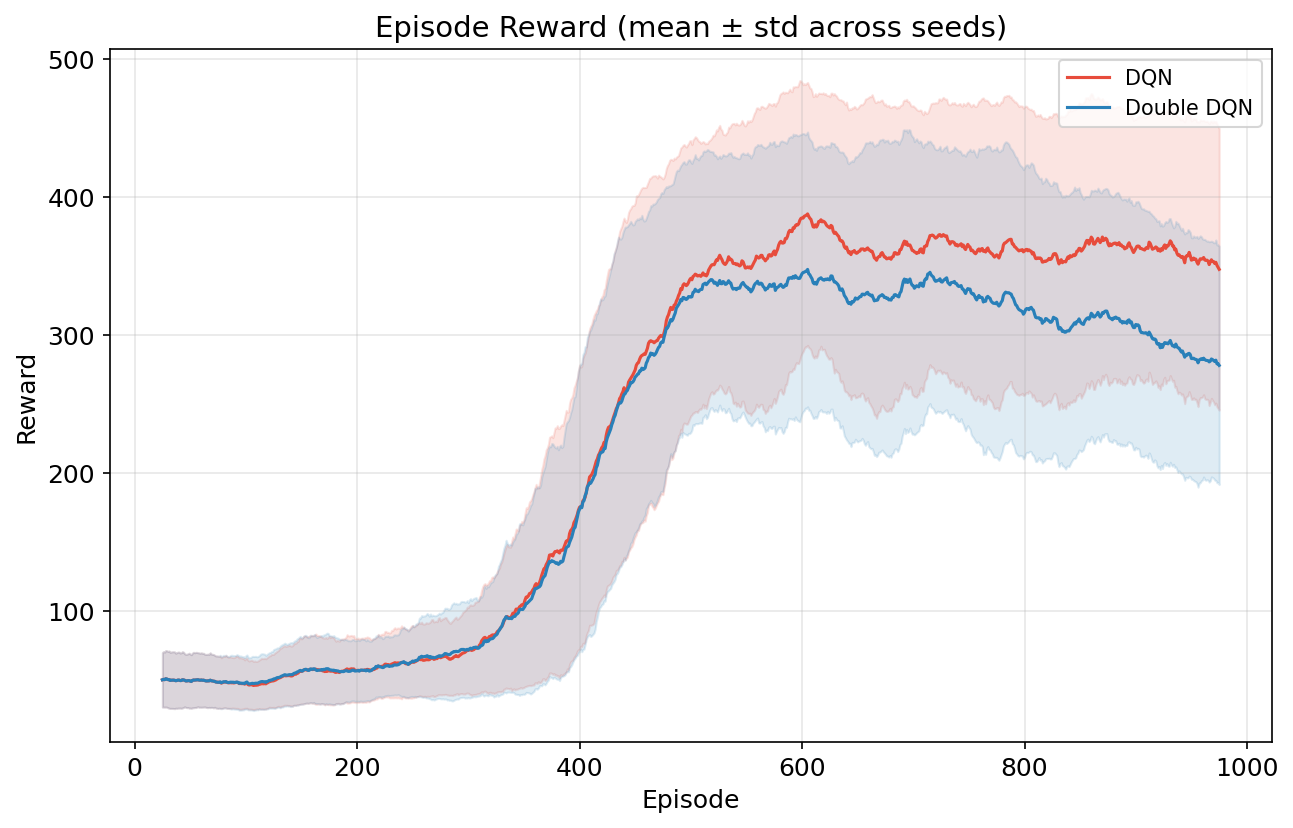
\includegraphics[width=\linewidth]{report_figures/phase2_after_reward_curve.png}
    \end{subfigure}
    \hfill
    \begin{subfigure}{0.48\textwidth}
        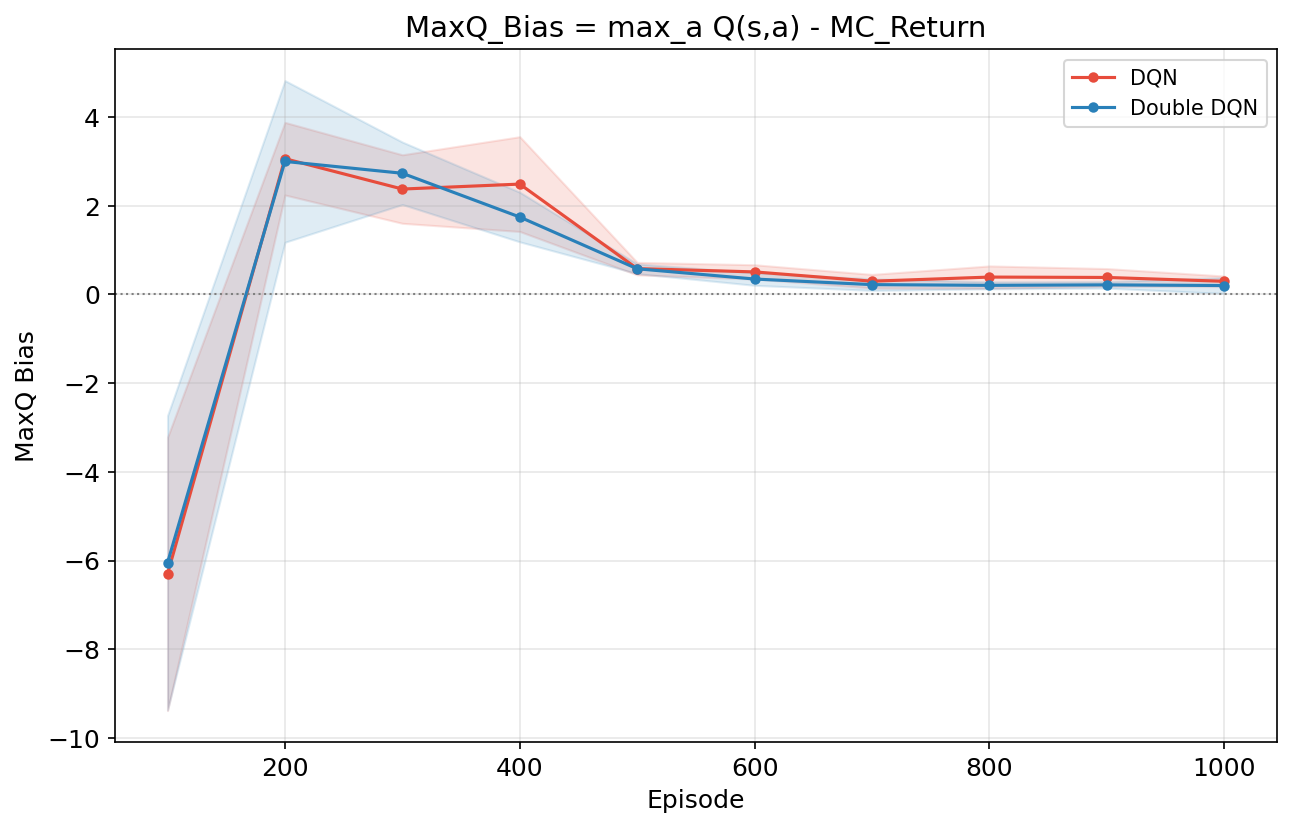
\includegraphics[width=\linewidth]{report_figures/phase2_after_maxq_bias_curve.png}
    \end{subfigure}
    \caption{Average Reward and MaxQ Bias after Hyperparameter Tuning}
    \label{fig:exp3_after}
\end{figure}

After implementing hyperparameter adjustments to mitigate the Deadly Triad, training stabilized sufficiently to observe meaningful bias behavior. Under these stable conditions, standard DQN achieved a higher final reward (355.7) but also exhibited a higher positive MaxQ Bias (+0.297). Double DQN exhibited a lower MaxQ Bias (+0.202), suggesting that decoupling action selection and evaluation continues to reduce overestimation even with complex neural network function approximation. However, the lower reward for Double DQN (285.4) in this specific experiment reinforces the observation that reduced bias does not inherently guarantee better short-term policy performance, particularly when training episodes are limited.

\section{Discussion}

\subsection{Overestimation Bias in Tabular RL}
The findings from Experiment 1 suggest that Q-Learning exhibits positive overestimation bias in a tabular setting. The max operator can amplify noisy action-value estimates, causing Q-Learning to move into the positive MaxQ Bias region over time. Double Q-Learning reduces this issue by separating action selection from value evaluation, resulting in a more conservative value estimate. However, the behavioral metrics show that value optimism does not translate directly into more aggressive control. In this experiment, Q-Learning produced a more spread and delayed-correction action pattern, while Double Q-Learning concentrated on a stronger corrective action, leading to longer pole stabilization.

\subsection{Deep RL Instability as an Implementation Challenge}
The transition to Deep RL introduced severe stability challenges, primarily driven by the Deadly Triad. The diagnostic results from the initial Deep RL implementation demonstrate that the combination of function approximation, bootstrapping, and off-policy replay can disrupt the learning dynamics. Instead of a gradual positive inflation, compounding errors caused massive divergence, rendering bias measurement difficult without intervention. This challenge necessitated significant hyperparameter tuning—specifically lowering the discount factor, accelerating target updates, and increasing gradient clipping—to mitigate the instability and anchor the Q-values to realistic bounds. It is important to note that hyperparameter tuning does not eliminate the Deadly Triad; it only reduces the rate at which errors accumulate, allowing the system to converge before divergence dominates.

\subsection{DQN vs Double DQN after Stabilization}
Once the Deadly Triad was mitigated, the expected bias mechanics re-emerged. The stabilized Deep RL comparison suggests that Double DQN maintains a lower MaxQ Bias (+0.202) compared to standard DQN (+0.297) even under function approximation. This supports the theoretical premise that the double estimator technique reduces bias in both the tabular and function approximation settings tested in this project. The gap is notably narrower than in the tabular setting, likely due to neural network generalization and the specific hyperparameter constraints applied to ensure stability.

\subsection{Bias Reduction versus Policy Performance}
A consistent theme across both tabular and deep experiments is that value-estimation bias and policy performance are related but not identical. In the tabular experiment, Double Q-Learning achieved both lower bias and slightly higher average reward (67.59 vs 63.08), suggesting that reducing overestimation can improve policy quality when the environment allows direct value observation. However, in the stabilized Deep RL comparison, the relationship reversed: DQN achieved higher short-term reward while Double DQN achieved lower MaxQ Bias. This indicates that the effect of bias reduction on policy performance is setting-dependent. Lower bias is desirable for value accuracy, but it does not automatically guarantee better short-term policy performance in every setting, particularly when function approximation and limited training episodes are involved.

\subsection{Connection to Theory and Literature}
The empirical results align well with foundational reinforcement learning literature. The positive bias observed in Experiment 1 practically illustrates the statistical consequences of Jensen's inequality when applying a max operator over noisy estimates. The success of Double Q-Learning and Double DQN in reducing this bias supports the double estimator theory proposed by van Hasselt. Additionally, the divergence observed before tuning is consistent with the instability described by the Deadly Triad, highlighting why modern Deep RL relies heavily on careful hyperparameter tuning and stabilizing architectural features.

\section{Limitations and Future Work}
While the experiments provided empirical evidence of overestimation bias and its reduction, several limitations should be noted. The \texttt{Stabilize-Isaac-Cartpole-v0} environment relies on a discretized action space consisting of only five levels, which may not capture the complexities of full continuous control. Furthermore, the training limit in the stabilized Deep RL comparison may have been insufficient for Double DQN to fully converge, potentially penalizing its more conservative learning rate compared to DQN. Finally, the specific hyperparameters tuned to mitigate the Deadly Triad were selected for immediate stability rather than optimized through an exhaustive grid search, meaning the relationship between parameters like learning rate, target update interval, and bias remains a subject for further exploration.

\textbf{Future Work:} 
The original proposal's scope included Prioritized Experience Replay (PER). Implementing PER alongside the stabilized Double DQN architecture is a logical next step to determine if intelligent sampling can accelerate Double DQN's conservative convergence rate. Exploring decaying learning rates and testing these algorithms in more complex environments with higher inherent noise (such as LunarLander) will help further validate the generalizability of these findings.

\newpage
\section{Conclusion}
This study traced the manifestation and mitigation of overestimation bias from Tabular Q-Learning to Deep Q-Networks. The empirical results suggest that while the double estimator approach reduces positive bias in both the tabular and deep RL settings examined in this project, the transition to function approximation introduces critical stability challenges. The Deadly Triad can heavily influence training dynamics, requiring careful hyperparameter tuning to mitigate divergence before meaningful bias analysis can occur. Ultimately, the findings indicate that while Double DQN provides a more conservative and less overestimated value estimate under the current setup, absolute policy performance remains dependent on the training context. Accurate value estimation is a fundamental goal, but it is not the sole determinant of short-term success in Reinforcement Learning.

\end{document}
